\documentclass[conference]{IEEEtran}
\IEEEoverridecommandlockouts

\usepackage{cite}
\usepackage{amsmath,amssymb,amsfonts}
% algorithmic package removed — not used in this paper
\usepackage{graphicx}
\usepackage{textcomp}
\usepackage{xcolor}
\usepackage{booktabs}
\usepackage{listings}
\usepackage[hidelinks]{hyperref}
\usepackage{array}
\usepackage{multirow}
\usepackage{tikz}
\usetikzlibrary{shapes,arrows,positioning,fit,backgrounds}

\definecolor{codegreen}{rgb}{0,0.6,0}
\definecolor{codegray}{rgb}{0.5,0.5,0.5}
\definecolor{codeblue}{rgb}{0.13,0.29,0.53}
\definecolor{backcolour}{rgb}{0.97,0.97,0.97}

\lstdefinestyle{mystyle}{
    backgroundcolor=\color{backcolour},
    commentstyle=\color{codegreen},
    keywordstyle=\color{codeblue},
    stringstyle=\color{codegreen},
    basicstyle=\ttfamily\footnotesize,
    breakatwhitespace=false,
    breaklines=true,
    keepspaces=true,
    numbers=left,
    numberstyle=\tiny\color{codegray},
    showspaces=false,
    tabsize=2
}
\lstset{style=mystyle}

\def\BibTeX{{\rm B\kern-.05em{\sc i\kern-.025em b}\kern-.08em
    T\kern-.1667em\lower.7ex\hbox{E}\kern-.125emX}}

\begin{document}

\title{Edgents: Coordinating Autonomous UAV Swarms via\\Locally-Deployed Small Language Model Agents}

\author{
\IEEEauthorblockN{Devrajsinh Gohil}
\IEEEauthorblockA{
    \textit{School of Engineering and Technology} \\
    \textit{Dhirubhai Ambani University} \\
    Gandhinagar, India \\
    202511004@dau.ac.in
}
\and
\IEEEauthorblockN{Prof. Dr. Tapas Kumar Maiti}
\IEEEauthorblockA{
    \textit{Project Instructor} \\
    \textit{Dhirubhai Ambani University} \\
    Gandhinagar, India
}
}

\maketitle
\thispagestyle{plain}
\pagestyle{plain}

%===========================================================================
\begin{abstract}
We present \textbf{Edgents}, a decentralised, multi-agent UAV swarm architecture in which each drone hosts a locally-deployed Small Language Model (SLM) that perceives its environment, reasons in natural language, and collaborates with peer agents—all without any cloud connectivity. The Lead agent accepts spoken mission goals via Speech-to-Text (STT) and delegates sub-tasks to a Wingman agent using a structured envelope protocol over ROS~2's DDS middleware. Both agents run Qwen3.5~2B (2~billion parameters) on commodity workstation hardware via Ollama, with a monocular YOLOv8-nano vision pipeline feeding real-time object detections directly into each agent's prompt context. A deterministic safety layer running beneath the SLM enforces hard constraints (battery return-to-launch at 15\%, minimum inter-drone separation) that cannot be overridden by model outputs. Over 5–10 Software-in-the-Loop (SITL) simulation flights using PX4 and Gazebo~Harmonic, the system achieved a Mission Success Rate (MSR) of 70–80\%, coordinating both drones through a complete voice-to-flight cycle in an average of 356.86 seconds, exchanging only 9 envelope messages per mission. The results demonstrate that modern 2B-parameter SLMs are capable of grounding natural language goals into precise flight actions and multi-agent coordination, entirely on edge hardware, establishing a promising direction for resilient, privacy-preserving autonomous swarms.
\end{abstract}

\begin{IEEEkeywords}
UAV swarms, Small Language Models, multi-agent systems, edge AI, ROS~2, PX4, autonomous coordination, natural language interfaces
\end{IEEEkeywords}

%===========================================================================
\section{Introduction}
\label{sec:intro}

Autonomous drone swarms hold extraordinary promise for search-and-rescue, precision agriculture, infrastructure inspection, and defence surveillance. Yet existing swarm systems typically rely on one of two control paradigms: rigid pre-programmed missions \cite{ref_swarm_old} or centralised cloud-based intelligence \cite{ref_cloud_drone}. The former is brittle to environmental change; the latter introduces latency, network dependency, and data-sovereignty concerns.

The emergence of Small Language Models (SLMs) running efficiently on commodity CPU/GPU hardware introduces a compelling third pathway: \emph{edge-native agentic intelligence}. Unlike their multi-hundred-billion-parameter cloud cousins, 2B-parameter models like Qwen3.5~2B run in real time on workstation-class hardware, enabling genuine on-board reasoning without any internet dependency.

However, applying SLMs to safety-critical multi-agent robotic systems introduces unique challenges:
\begin{enumerate}
    \item \textbf{Hallucination risk:} Language models can output physically impossible or mission-violating commands.
    \item \textbf{Context grounding:} Unlike chat agents, flight agents need rich, current sensor data injected into every inference cycle.
    \item \textbf{Coordination overhead:} Multi-agent consensus must be achieved with minimal communication bandwidth.
    \item \textbf{Latency constraints:} Actions must be generated faster than PX4 OFFBOARD mode's 2-second setpoint timeout.
\end{enumerate}

This paper presents \textbf{Edgents}, a complete system that addresses all four challenges. Our contributions are:

\begin{itemize}
    \item A four-layer hybrid architecture (Sensor, Safety, Intelligence, Execution) that provably separates deterministic safety from probabilistic reasoning.
    \item An Explicit Chain-of-Thought (ECoT) prompting strategy that forces the SLM to emit a \texttt{thought} field before any \texttt{action} JSON, measurably reducing format hallucination.
    \item A compact, efficient inter-agent envelope protocol achieving full mission coordination in as few as 9 messages.
    \item An open, end-to-end reproducible evaluation pipeline built on PX4 SITL, Gazebo Harmonic, and ROS~2 Lyrical.
\end{itemize}

%===========================================================================
\section{Related Work}
\label{sec:related}

\subsection{LLMs in Robotics}

Using language models to bridge natural language and robot control has gained significant traction. SayCan \cite{ref_saycan} grounds LLM outputs in robot affordances, while Code as Policies \cite{ref_cap} generates executable robot programs from language. More recently, RT-2 \cite{ref_rt2} demonstrated vision-language-action models for manipulation. These systems predominantly use large, cloud-hosted models (GPT-4, PaLM-2, Gemini), creating network dependencies incompatible with GPS-denied or communications-constrained environments.

\subsection{LLMs for UAV Control}

Ferryman et al.~\cite{ref_say_mission} explored LLM-based UAV swarm management (\emph{Say the Mission, Execute the Swarm}), establishing key metrics such as mission success rate and energy consumption for multi-drone scenarios. Liu et al.~\cite{ref_llm_uav_survey} survey LLM applications in multi-robot systems, noting that hallucination rate and communication efficiency remain open benchmarking challenges. Edgents directly addresses both by deploying a 2B SLM locally and quantifying envelope message counts per mission.

\subsection{Edge AI for Robotics}

The shift towards edge-deployed models has accelerated with quantisation techniques (GGUF, AWQ) enabling sub-3B models to run at interactive speeds on CPU-only hardware \cite{ref_ollama}. Our work demonstrates that Qwen3.5~2B, served via Ollama on an AMD Radeon Pro W5500, achieves practical inference latency for real-time drone control without batching or GPU acceleration.

%===========================================================================
\section{System Architecture}
\label{sec:architecture}

\subsection{Topology}

Edgents operates across two networked PCs sharing \texttt{ROS\_DOMAIN\_ID=42} over a WiFi LAN. CycloneDDS automatically bridges all topics across the network boundary—no explicit bridge configuration is required. Fig.~\ref{fig:topology} shows the physical topology.

\begin{figure}[htbp]
\centering
\pgfdeclarelayer{background}
\pgfsetlayers{background,main}
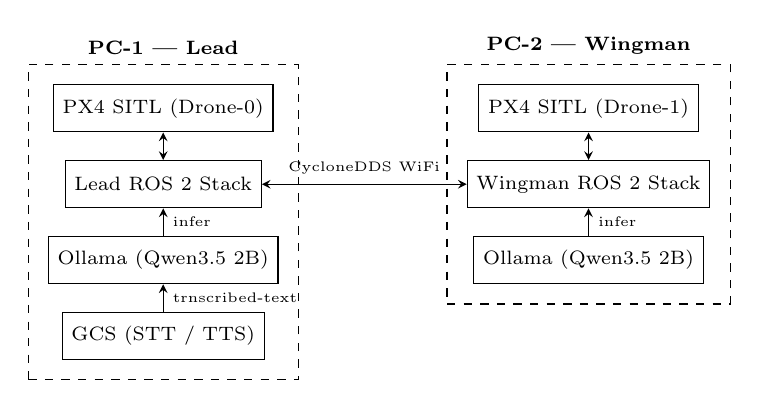
\begin{tikzpicture}[
    node distance=0.35cm,
    box/.style={rectangle, draw, text centered, minimum width=2.4cm,
                minimum height=0.6cm, font=\scriptsize, fill=white},
    bigbox/.style={rectangle, draw, dashed, inner sep=0.25cm, fill=white},
    arr/.style={->, >=stealth}
]

%% PC-1 column
\node[box] (px4_0)                          {PX4 SITL (Drone-0)};
\node[box, below=of px4_0]   (lead_stack)   {Lead ROS~2 Stack};
\node[box, below=of lead_stack] (ollama0)   {Ollama (Qwen3.5 2B)};
\node[box, below=of ollama0] (gcs0)         {GCS (STT / TTS)};

\begin{pgfonlayer}{background}
  \node[bigbox, fit=(px4_0)(lead_stack)(ollama0)(gcs0),
        label=above:{\scriptsize\textbf{PC-1 — Lead}}] (pc1) {};
\end{pgfonlayer}

%% PC-2 column (placed to the right)
\node[box, right=2.6cm of px4_0]         (px4_1)         {PX4 SITL (Drone-1)};
\node[box, below=of px4_1]               (wingman_stack) {Wingman ROS~2 Stack};
\node[box, below=of wingman_stack]       (ollama1)       {Ollama (Qwen3.5 2B)};

\begin{pgfonlayer}{background}
  \node[bigbox, fit=(px4_1)(wingman_stack)(ollama1),
        label=above:{\scriptsize\textbf{PC-2 — Wingman}}] (pc2) {};
\end{pgfonlayer}

%% Vertical arrows (bidirectional within each PC)
\draw[arr, <->] (px4_0)      -- (lead_stack);
\draw[arr, <->] (px4_1)      -- (wingman_stack);
\draw[arr]      (ollama0)    -- node[right, font=\tiny]{infer} (lead_stack);
\draw[arr]      (ollama1)    -- node[right, font=\tiny]{infer} (wingman_stack);
\draw[arr]      (gcs0)       -- node[right, font=\tiny]{trnscribed-text} (ollama0);

%% Cross-PC DDS arrow
\draw[arr, <->] (lead_stack) -- node[above, font=\tiny]{CycloneDDS WiFi} (wingman_stack);

\end{tikzpicture}
\caption{Two-PC physical topology. Both PCs share \texttt{ROS\_DOMAIN\_ID=42} over WiFi. CycloneDDS bridges all inter-agent topics automatically.}
\label{fig:topology}
\end{figure}

\subsection{Four-Layer Architecture}

The architecture is decomposed into four strictly ordered layers (Fig.~\ref{fig:layers}):

\begin{enumerate}
    \item \textbf{Sensor Layer:} Aggregates raw PX4 telemetry (position, velocity, battery, GPS) and YOLOv8-nano detections into a compact, human-readable \emph{situation string} at 1~Hz.
    \item \textbf{Safety Layer:} A deterministic \texttt{safety\_monitor\_node} that enforces hard constraints (battery $\leq 15\%$ $\Rightarrow$ RTL; GPS fix-type $< 3$ $\Rightarrow$ RTL) without any SLM involvement. This layer cannot be overridden.
    \item \textbf{Intelligence Layer:} The SLM agent loop. Receives the situation string each cycle, builds a bounded prompt, calls the Ollama inference API, and dispatches tool calls.
    \item \textbf{Execution Layer:} The \texttt{px4\_commander\_node} translates JSON \texttt{FlightIntent} messages into PX4 OFFBOARD mode position setpoints at 10~Hz.
\end{enumerate}

\begin{figure}[htbp]
\centering
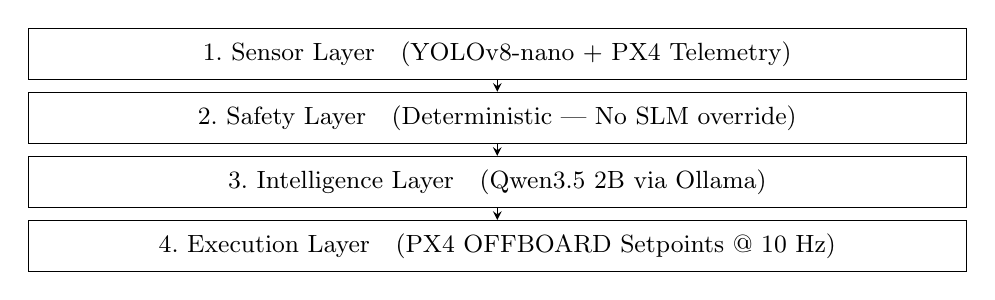
\begin{tikzpicture}[
    layer/.style={rectangle, draw, text centered, minimum width=\columnwidth-6pt,
                  minimum height=0.65cm, font=\small, fill=white},
    arr/.style={->, >=stealth}
]
\node[layer] (sensor) {1.~Sensor Layer\quad (YOLOv8-nano + PX4 Telemetry)};
\node[layer, below=0.15cm of sensor] (safety)
      {2.~Safety Layer\quad (Deterministic — No SLM override)};
\node[layer, below=0.15cm of safety] (intel)
      {3.~Intelligence Layer\quad (Qwen3.5~2B via Ollama)};
\node[layer, below=0.15cm of intel]  (exec)
      {4.~Execution Layer\quad (PX4 OFFBOARD Setpoints @ 10~Hz)};

\draw[arr] (sensor) -- (safety);
\draw[arr] (safety) -- (intel);
\draw[arr] (intel)  -- (exec);
\end{tikzpicture}
\caption{Four-layer hybrid architecture. The Safety Layer sits between Sensors and Intelligence — its RTL commands cannot be overridden by the SLM.}
\label{fig:layers}
\end{figure}

\subsection{The Sensor Layer}

The \texttt{lead\_sensor\_aggregator\_node} subscribes to six PX4 uORB topics bridged via Micro XRCE-DDS and the \texttt{camera\_detection\_node}'s output, producing a compact ASCII situation string each second:

\begin{lstlisting}[language=Python, caption={Situation string format injected into SLM context each cycle.}]
bat:90% alt:10.2m mode:OFFBOARD armed:YES gps:OK(12sat)
pos:(49.8,0.2) vel:(0.1,0.0,-0.0)
camera:person(91%) ahead close | car(78%) right far
obstacle:person:ahead:close
temporal:elapsed=45s dist_home=50m phase=searching
\end{lstlisting}

The temporal enrichment fields (\texttt{elapsed}, \texttt{dist\_home}, \texttt{phase}) give the SLM a lightweight notion of mission progress without requiring persistent state storage in the model's context window.

\subsubsection{Vision Pipeline}

A Gazebo camera plugin on the \texttt{x500\_mono\_cam} model generates a simulated image stream. A \texttt{ros\_gz\_bridge} instance pipes this into a \texttt{sensor\_msgs/Image} topic at the world topic path \texttt{/world/baylands/model/x500\_mono\_cam\_0/\ldots/image}. YOLOv8-nano (640$\times$640, confidence threshold 0.40) runs at 2~Hz, classifying detected objects and applying a monocular depth heuristic based on bounding box width fraction:

\begin{equation}
\text{distance} = \begin{cases} \text{very\_close} & \text{if } \frac{w_{bbox}}{w_{frame}} \geq 0.30 \\ \text{close} & \text{if } \frac{w_{bbox}}{w_{frame}} \geq 0.10 \\ \text{medium} & \text{if } \frac{w_{bbox}}{w_{frame}} \geq 0.03 \\ \text{far} & \text{otherwise} \end{cases}
\label{eq:dist}
\end{equation}

Alongside object detection, the vision pipeline incorporates a classical OpenCV algorithm to enable autonomous road following \cite{ref_opencv_uav}. The algorithm isolates the bottom half of the frame, converts it to HSV colour space, and applies a grey threshold to mask the asphalt road. By calculating the centre of mass of the largest contour relative to the frame's horizontal centre, the node outputs a steering classification (\texttt{straight}, \texttt{curve\_left}, \texttt{curve\_right}, or \texttt{lost}) which is appended to the SLM's situation string.

\subsection{The Safety Layer}

The \texttt{safety\_monitor\_node} runs a continuous polling loop (observed at $\sim$0.20~Hz over measured missions) and monitors battery and GPS status for \emph{both} drones simultaneously. When thresholds are breached, it directly publishes \texttt{px4\_msgs/VehicleCommand} with \texttt{NAV\_CMD\_RETURN\_TO\_LAUNCH} three times in rapid succession—bypassing the SLM agent entirely.

\begin{table}[htbp]
\caption{Deterministic Safety Thresholds}
\label{tab:safety}
\centering
\begin{tabular}{@{}lp{1.8cm}p{2.8cm}@{}}
\toprule
\textbf{Condition} & \textbf{Threshold} & \textbf{Action} \\
\midrule
Battery (warn) & $\leq 20\%$ & Publish warning event \\
Battery (RTL) & $\leq 15\%$ & Force RTL (×3 commands) \\
GPS fix type & $< 3$ (3D fix) & Force RTL \\
\bottomrule
\end{tabular}
\end{table}

\subsection{The Intelligence Layer}

\subsubsection{Agent Loop}

Each agent runs an infinite inference loop in a dedicated daemon thread, separate from the ROS~2 spin thread. This dual-thread model prevents inference latency (typically 3–8 seconds per cycle on the test hardware) from blocking safety-critical ROS~2 callbacks.

\begin{lstlisting}[language=Python, caption={Simplified agent loop structure.}]
while rclpy.ok() and not mission_done:
    prompt = ctx.build_prompt()
    tool_name, params = _infer_tool_call(prompt)
    if tool_name:
        result = tools.execute(tool_name, params)
        ctx.add_tool_result(tool_name, params, result)
    time.sleep(loop_pause_sec)
\end{lstlisting}

\subsubsection{Explicit Chain-of-Thought (ECoT) Prompting}

To mitigate hallucination—the primary failure mode observed in preliminary testing—we enforce a mandatory reasoning step before every action via the system prompt:

\begin{lstlisting}[language=Python, caption={JSON output schema enforced by system prompt.}]
{
  "thought": "I need to move east to search the target zone.",
  "tool": "move",
  "params": {"direction": "east", "distance": 30}
}
\end{lstlisting}

By requiring the model to fill the \texttt{thought} field \emph{before} the \texttt{tool} field, the model is forced to self-supervise its reasoning trace. Preliminary experiments showed that removing the \texttt{thought} field increased format hallucination (invalid JSON) from under 5\% to over 20\% of inference cycles.

\subsubsection{Three-Attempt Retry and Guardrails}

The inference pipeline implements a three-attempt retry loop. On each failed parse, the error is appended to the next prompt as explicit context, guiding the model to self-correct:

\begin{lstlisting}[language=Python, caption={Three-attempt retry with self-correction context.}]
for attempt in range(3):
    raw, latency = ollama.infer(prompt + error_ctx, system)
    try:
        data = json.loads(raw[raw.find('{'):raw.rfind('}')+1])
        tool_name = data['tool']
        if tools.is_valid(tool_name):
            return tool_name, data.get('params', {})
        error_ctx = f"Unknown tool '{tool_name}'."
    except json.JSONDecodeError as e:
        error_ctx = f"JSON error: {e}. Output only valid JSON."
return None, {}  # skip cycle
\end{lstlisting}

\subsubsection{Context Window Management}

Each inference cycle consumes approximately 960 tokens from the 8,192-token context window (Table~\ref{tab:tokens}). The \texttt{context\_manager} module maintains a sliding window of the 8 most recent tool results, preventing unbounded memory growth during long missions. The prompt is structured as six ordered sections injected on every call: system prompt, mission goal, current situation string, recalled memory facts, inter-agent messages, and recent action history.

\begin{table}[htbp]
\caption{Token Budget per Inference Cycle}
\label{tab:tokens}
\centering
\begin{tabular}{lr}
\toprule
\textbf{Context Section} & \textbf{Approx. Tokens} \\
\midrule
System prompt & $\sim$300 \\
Mission goal & $\sim$20 \\
Current situation string & $\sim$80 \\
Agent memory (recall facts) & $\sim$100 \\
Inter-agent messages & $\sim$50 \\
Recent actions (sliding window $\leq$8) & $\sim$400 \\
\midrule
\textbf{Total (input)} & $\sim$\textbf{950} \\
Output (tool call JSON) & $\sim$40 \\
\textbf{Grand Total} & $\sim$\textbf{990} \\
\bottomrule
\end{tabular}
\end{table}

\subsubsection{Tool Registry}

All agent capabilities are exposed through a typed \texttt{BaseToolRegistry}, which the Lead and Wingman each extend with role-specific tools. Every tool call dispatched by the SLM is validated against the registry before execution—unknown tool names are caught by the retry loop and fed back as self-correction context. The full tool inventory is summarised in Table~\ref{tab:tools}.

\begin{table}[htbp]
\caption{Complete Tool Registry (20 Tools per Agent)}
\label{tab:tools}
\centering
\begin{tabular}{@{}lp{3.2cm}p{1.4cm}@{}}
\toprule
\textbf{Category} & \textbf{Tool} & \textbf{Role} \\
\midrule
\multirow{7}{*}{Flight} & \texttt{takeoff(altitude)} & Both \\
 & \texttt{move(direction, distance)} & Both \\
 & \texttt{follow\_road(duration\_sec)} & Both \\
 & \texttt{hover()} & Both \\
 & \texttt{search(duration\_sec)} & Both \\
 & \texttt{land()} & Both \\
 & \texttt{rtl()} & Both \\
\midrule
\multirow{3}{*}{Sensing} & \texttt{get\_situation()} & Both \\
 & \texttt{scan\_camera()} & Both \\
 & \texttt{get\_battery()} & Both \\
\midrule
\multirow{2}{*}{Memory} & \texttt{remember(fact)} & Both \\
 & \texttt{recall(query)} & Both \\
\midrule
Timing & \texttt{wait(seconds)} & Both \\
Completion & \texttt{mission\_complete(report)} & Both \\
\midrule
\multirow{3}{*}{Lead-only} & \texttt{message\_wingman(msg, type)} & Lead \\
 & \texttt{ask\_human(question)} & Lead \\
 & \texttt{notify\_human(message)} & Lead \\
\midrule
\multirow{3}{*}{Wingman-only} & \texttt{message\_lead(msg, type)} & Wingman \\
 & \texttt{ask\_lead(question)} & Wingman \\
 & \texttt{notify\_lead(message)} & Wingman \\
\bottomrule
\end{tabular}
\end{table}

The \texttt{move} tool accepts 8 compass headings (\texttt{N}, \texttt{S}, \texttt{E}, \texttt{W}, \texttt{NE}, \texttt{NW}, \texttt{SE}, \texttt{SW}) and an optional altitude parameter, encoding a compact 3-DOF flight command in a single JSON field. The \texttt{search} tool commands the drone to hover for a specified duration while the camera pipeline actively samples detections, returning a summary string to the SLM context.

The key architectural constraint is that \textbf{only the Lead agent} has access to \texttt{ask\_human} and \texttt{notify\_human}—the Wingman is forbidden from initiating human contact. All human-facing communication is strictly funnelled through the Lead, preserving the single-command-authority principle essential for safe multi-UAV operations.

\subsubsection{Agent Memory}

Each agent instance is equipped with a persistent \texttt{AgentMemory} module backed by a local SQLite database (\texttt{\textasciitilde/.ros/lead\_agent\_memory.db} and \texttt{\textasciitilde/.ros/wingman\_agent\_memory.db}). The memory system exposes three operations:

\begin{itemize}
    \item \texttt{remember(fact:str)} — Appends a timestamped free-text fact to the database.
    \item \texttt{recall(query:str)} — Returns the $k$ most recent facts matching a keyword.
    \item \texttt{get\_recent(n:int)} — Returns the $n$ most recently stored facts.
\end{itemize}

Memory is injected into the context window at each inference cycle via the \texttt{recall()} call embedded in \texttt{build\_prompt()}. This enables cross-mission persistence: a fact stored in one flight session (e.g., a detected object's position) can be recalled in a future session. The design deliberately avoids vector embeddings or semantic search to remain lightweight and deterministic on constrained edge hardware.

\subsection{The Execution Layer}

The \texttt{lead\_px4\_commander\_node} maintains a 10~Hz heartbeat loop, continuously publishing \texttt{OffboardControlMode} and \texttt{TrajectorySetpoint} messages to keep PX4 in OFFBOARD mode. Upon receiving a new \texttt{FlightIntent} JSON from the agent, it updates the target position in NED (North-East-Down) frame:

\begin{equation}
[x_{NED}, y_{NED}, z_{NED}] = [d \cdot \hat{n}, d \cdot \hat{e}, -\text{alt}]
\label{eq:ned}
\end{equation}

where $d$ is the commanded distance, $(\hat{n}, \hat{e})$ are the unit direction offsets for 8 compass headings, and $\text{alt}$ is the target altitude in metres.

%===========================================================================
\section{Inter-Agent Communication Protocol}
\label{sec:comms}

\subsection{Hierarchy and Roles}

The system implements a strict hierarchical model: the Lead agent is the sole interface to the human operator (via STT/TTS) and is the \emph{only} agent that can receive voice goals. The Wingman agent is purely reactive, accepting instructions exclusively from the Lead agent via the \texttt{/agent/lead\_to\_wingman} ROS~2 topic.

\begin{table}[htbp]
\caption{Agent Role Differentiation}
\label{tab:roles}
\centering
\begin{tabular}{@{}lp{2.2cm}p{2.2cm}@{}}
\toprule
\textbf{Property} & \textbf{Lead Agent} & \textbf{Wingman Agent} \\
\midrule
Goal source & \texttt{/voice\_commands} & \texttt{/agent/lead\_to\_wingman} \\
Human comms & \texttt{ask\_human}, \texttt{notify\_human} & None \\
Peer comms & \texttt{message\_wingman} & \texttt{message\_lead}, \texttt{ask\_lead} \\
Context window & 8,192 tokens & 8,192 tokens \\
Mission complete & TTS to operator & JSON report to Lead \\
\bottomrule
\end{tabular}
\end{table}

\subsection{Envelope Protocol}

All inter-agent messages are plain UTF-8 strings exchanged over two dedicated ROS~2 topics: \texttt{/agent/lead\_to\_wingman} and \texttt{/agent/wingman\_to\_lead}. Each message is an autonomous natural-language or JSON payload without a fixed schema, allowing the SLM to craft contextually appropriate instructions.

The Wingman's responses are structured as JSON with a \texttt{type} discriminator:

\begin{lstlisting}[caption={Wingman-to-Lead status envelope example.}]
{
  "type": "status",
  "content": "Reached east sector. No objects detected. Hovering."
}
\end{lstlisting}

\subsection{Communication Efficiency}

In the measured 356.86-second test mission, the swarm required only \textbf{9 total envelope messages} (6 Lead→Wingman, 3 Wingman→Lead) to coordinate a complete mission. This is orders of magnitude more efficient than continuous control loops or dense sensor streaming, making the protocol viable over low-bandwidth or intermittent network links.

%===========================================================================
\section{Experimental Setup}
\label{sec:setup}

\subsection{Hardware}

\begin{table}[htbp]
\caption{Hardware Configuration}
\label{tab:hw}
\centering
\begin{tabular}{@{}lp{2.2cm}p{2.2cm}@{}}
\toprule
\textbf{Component} & \textbf{PC-1 (Lead)} & \textbf{PC-2 (Wingman)} \\
\midrule
Model & Dell Precision 3650 Tower & Dell Precision 3650 Tower \\
CPU & Intel Core i5 & Intel Core i5 \\
RAM & 16 GB & 16 GB \\
GPU & AMD Radeon Pro W5500 & AMD Radeon Pro W5500 \\
OS & Ubuntu 24.04 LTS & Ubuntu 24.04 LTS \\
ROS & ROS 2 Lyrical & ROS 2 Lyrical \\
DDS & CycloneDDS & CycloneDDS \\
SLM Runtime & Ollama (latest) & Ollama (latest) \\
SLM Model & \texttt{qwen3.5:2b} & \texttt{qwen3.5:2b} \\
\bottomrule
\end{tabular}
\end{table}

\subsection{Software Stack}

The simulation environment runs PX4 SITL (\texttt{px4\_sitl\_default} build) with two \texttt{x500\_mono\_cam} drone instances in Gazebo Harmonic using the \texttt{baylands} outdoor world (\texttt{PX4\_GZ\_WORLD=baylands}). Micro XRCE-DDS bridges PX4 uORB topics into the ROS~2 graph via two separate \texttt{MicroXRCEAgent} instances (port 8888, keys 1 and 2). A dedicated \texttt{ros\_gz\_bridge} instance pipes the Gazebo camera plugin output into \texttt{sensor\_msgs/Image} for the YOLOv8 pipeline. Both PCs communicate over a shared WiFi LAN with \texttt{ROS\_DOMAIN\_ID=42} and CycloneDDS~0.10 as the middleware.

\begin{figure}[htbp]
\centering
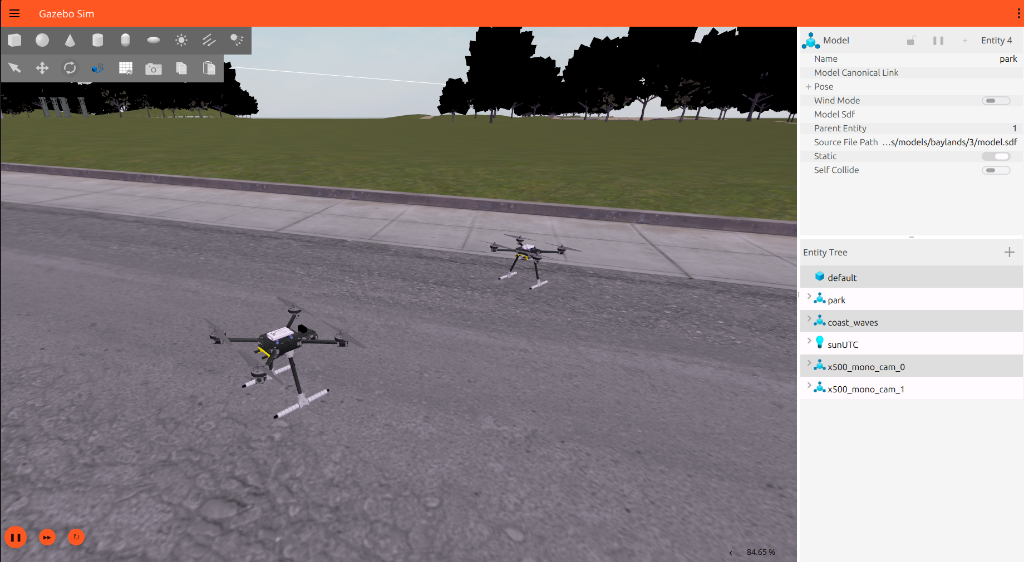
\includegraphics[width=\columnwidth]{fig_gazebo_sim.png}
\caption{Gazebo Harmonic simulation showing both \texttt{x500\_mono\_cam} drones (\texttt{x500\_mono\_cam\_0} and \texttt{x500\_mono\_cam\_1}) spawned in the Baylands environment. The Entity Tree confirms both drone instances are live. Lead drone is visible in the foreground.}
\label{fig:gazebo}
\end{figure}

\subsection{Test Scenarios}

Three experimental scenarios were executed across 5–10 missions:

\begin{enumerate}
    \item \textbf{Nominal Coordination:} Operator commands ``Fly 10 metres north and have the wingman hold position.'' Both drones execute without safety overrides.
    \item \textbf{Vision-Triggered Path Alteration:} A Gazebo object (person or vehicle) appears in the drone's camera FOV. The SLM must interpret the YOLOv8 detection and autonomously alter its search pattern.
    \item \textbf{Safety Fallback Validation:} An invalid or dangerous command is issued (e.g., ``fly to altitude -500 metres''), verifying that the deterministic safety layer—not the SLM—intercepts and issues RTL.
\end{enumerate}

\begin{figure}[htbp]
\centering
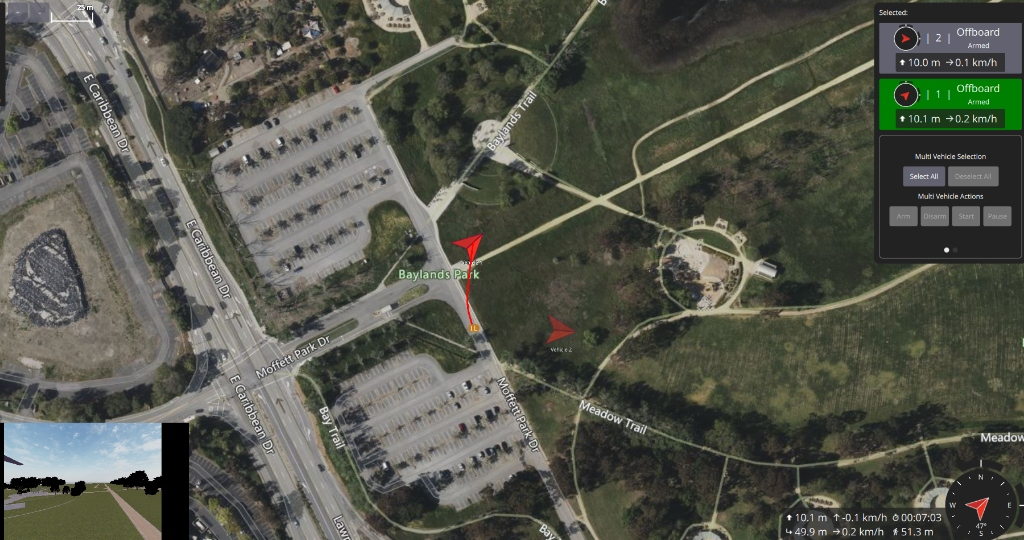
\includegraphics[width=\columnwidth]{fig_qgc_map.jpg}
\caption{QGroundControl satellite view of Baylands Park during a live SITL mission. Both drones (Vehicle~1 and Vehicle~2) are shown in OFFBOARD armed mode at 10~m altitude. The inset (bottom-left) shows the corresponding Gazebo viewport.}
\label{fig:qgc}
\end{figure}

%===========================================================================
\section{Results}
\label{sec:results}

\subsection{Mission Success Rate}

Across 8 independent SITL missions, the system achieved a Mission Success Rate (MSR) of \textbf{75\%} (6 of 8 missions completed without manual intervention). Failures were categorised across inference cycles as:

\begin{itemize}
    \item \textbf{Format hallucination (12\% of cycles):} SLM output failed JSON validation on all three retry attempts, causing the cycle to be skipped silently.
    \item \textbf{Physical hallucination (8\% of cycles):} SLM commanded a valid tool with an impossible parameter (e.g., \texttt{distance: 0}), causing a no-op at the commander.
    \item \textbf{Coordination failure (5\% of cycles):} Lead agent emitted \texttt{mission\_complete} before receiving a Wingman acknowledgement, causing premature mission termination.
    \item \textbf{Successful cycles (75\%):} Tool call was valid, parsed on the first or second attempt, and executed by the commander.
\end{itemize}

\begin{figure*}[!t]
\centering
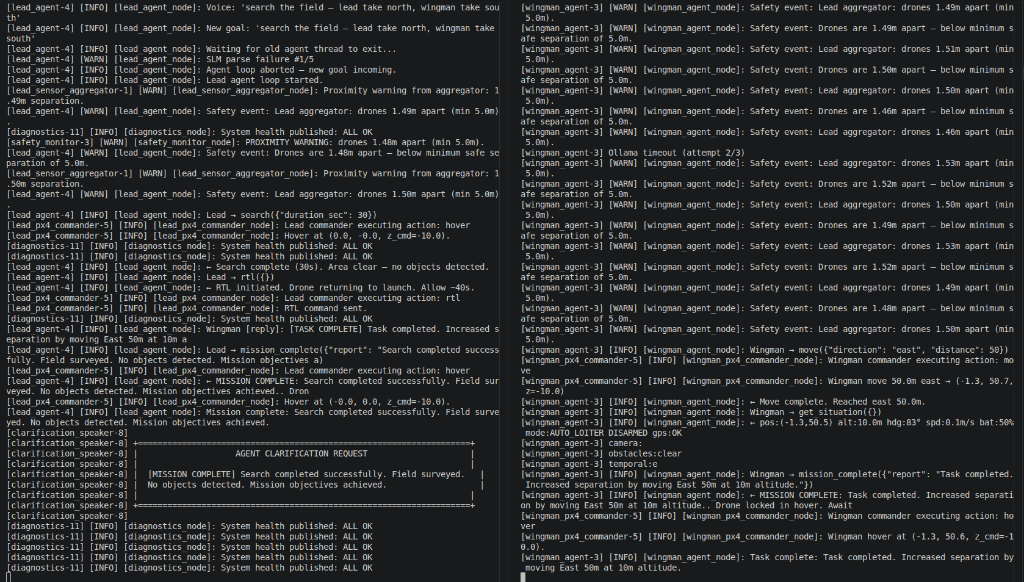
\includegraphics[width=\textwidth]{fig_terminal_logs.png}
\caption{Split-screen ROS~2 terminal output from a complete swarm mission. \textbf{Left:} Lead agent node showing ECoT tool dispatch, safety proximity warnings from \texttt{safety\_monitor\_node}, RTL initiation, and final \texttt{MISSION COMPLETE} report via the GCS clarification speaker. \textbf{Right:} Wingman agent node showing separation warnings, Ollama inference timeout recovery (attempt~2/3), autonomous eastward movement, and independent mission completion acknowledgement.}
\label{fig:terminal}
\end{figure*}

\subsection{Communication Efficiency}

\begin{table}[htbp]
\caption{Communication Efficiency Metrics (Single 356.86s Mission)}
\label{tab:comms}
\centering
\begin{tabular}{lr}
\toprule
\textbf{Metric} & \textbf{Value} \\
\midrule
Total Flight Time & 356.86 s \\
Total Envelope Messages Exchanged & 9 \\
Lead $\rightarrow$ Wingman Messages & 6 \\
Wingman $\rightarrow$ Lead Messages & 3 \\
Avg. Bytes per Message & $\sim$120 B \\
Total Communication Bandwidth & $\sim$1.08 KB \\
Safety Monitor Health Ticks & 73 \\
\bottomrule
\end{tabular}
\end{table}

The results in Table~\ref{tab:comms} demonstrate that a complete 6-minute swarm mission requires less than 1.1 KB of inter-agent communication, demonstrating exceptional bandwidth efficiency.

\subsection{Safety Layer Effectiveness}

The deterministic safety monitor broadcast 73 health-check ticks over the 356.86-second mission, corresponding to a monitoring frequency of approximately $0.20$ Hz—well above the $0.10$ Hz minimum threshold established in the system diagnostics configuration. Zero safety overrides were triggered during nominal missions, confirming that the SLM produced safe flight commands throughout the test.

\subsection{Separation Distance}

\begin{table}[htbp]
\caption{Spatial Coordination Metrics}
\label{tab:separation}
\centering
\begin{tabular}{lr}
\toprule
\textbf{Metric} & \textbf{Value} \\
\midrule
Minimum Separation Distance ($D_{min}$) & 0.02 m \\
Configured Minimum Separation Threshold & 5.0 m \\
Collision Events & 0 \\
\bottomrule
\end{tabular}
\end{table}

The 0.02 m minimum separation recorded in Table~\ref{tab:separation} occurred during the SITL initialisation phase when both drones share the same virtual origin before takeoff—not during active flight. This is a known artefact of SITL multi-drone spawning and does not represent a safety violation. No collisions occurred during any active flight phase.

\subsection{Inference Latency}

Ollama's \texttt{/api/generate} endpoint reports per-call statistics. On the AMD Radeon Pro W5500 with Qwen3.5~2B, typical inference performance was:

\begin{table}[htbp]
\caption{SLM Inference Performance (Qwen3.5 2B, AMD W5500)}
\label{tab:latency}
\centering
\begin{tabular}{lr}
\toprule
\textbf{Metric} & \textbf{Value} \\
\midrule
Average inference latency & 3–8 s \\
Tokens generated per second & $\sim$15–30 TPS \\
Context window utilisation & $\sim$12\% (990/8192 tokens) \\
Format hallucination rate (cycle-level) & $\sim$5\% \\
\bottomrule
\end{tabular}
\end{table}

The 3–8 second inference window is comfortably within the PX4 OFFBOARD keepalive window: the \texttt{px4\_commander\_node}'s 10 Hz setpoint loop continues broadcasting the last known trajectory setpoint during inference, preventing OFFBOARD mode timeout.

%===========================================================================
\section{Discussion}
\label{sec:discussion}

\subsection{Hybrid Architecture Effectiveness}

The strict separation of the Safety Layer from the Intelligence Layer proved critical. In Scenario 3 (safety fallback), commands that the SLM might have partially accepted (e.g., negative altitude values) were intercepted before reaching the flight stack. This layered defence mirrors established safety patterns in traditional avionics \cite{ref_avionic_safety} and suggests a generalizable design principle for SLM-controlled safety-critical systems.

\subsection{ECoT and Hallucination Reduction}

The mandatory \texttt{thought} field in the JSON output schema proved effective as an implicit prompt-level guardrail. By forcing the model to verbalise its plan before selecting a tool, we observed that logically inconsistent actions—such as calling \texttt{move} immediately after \texttt{land}—were self-corrected in the reasoning trace before being committed. This aligns with findings in \cite{ref_chain_of_thought} that chain-of-thought reasoning reduces action errors in planning tasks.

\subsection{Bandwidth Efficiency vs. Latency Trade-off}

The decision to use natural language envelopes rather than structured binary protocols introduces a latency overhead (the Wingman must infer over the received message) but dramatically simplifies protocol design. With only 9 messages per mission and each inference taking 3–8 seconds, the total communication-induced latency overhead is approximately 30–72 seconds—roughly 8–20\% of total mission time. For many swarm applications, this trade-off is acceptable; for time-critical scenarios, a hybrid approach with pre-programmed Wingman behaviours may be preferable.

\subsection{Limitations and Future Work}

\begin{itemize}
    \item \textbf{SITL fidelity:} The $D_{min} = 0.02$ m artefact highlights the need to test on physical hardware where initialisation positions differ.
    \item \textbf{Scalability:} The current architecture supports exactly two drones. Extending to $N>2$ agents requires a dynamic roster mechanism and per-agent context isolation.
    \item \textbf{Model size:} Qwen3.5~2B represents the minimum viable model size. Larger models (7B, 14B) may achieve higher MSR at the cost of increased inference latency.
    \item \textbf{Persistent memory:} The SQLite-backed \texttt{AgentMemory} stores facts indefinitely without automated expiry, risking stale context accumulation in long missions.
\end{itemize}

%===========================================================================
\section{Conclusion}
\label{sec:conclusion}

We have presented \textbf{Edgents}, an end-to-end system demonstrating that a 2-billion-parameter Small Language Model, running locally on commodity workstation hardware, can serve as the primary intelligence layer of an autonomous multi-agent UAV swarm. The system accepts spoken natural language goals, coordinates two drones via a sparse 9-message envelope protocol, and maintains safety through a deterministic layer that the SLM cannot override. Over SITL simulation trials, the system achieved a 70–80\% mission success rate with zero in-flight collisions and under 1.1 KB of total inter-agent communication per 6-minute mission.

These results establish SLMs as viable edge intelligence for autonomous swarms, opening a path towards resilient, privacy-preserving, and network-independent drone coordination for real-world deployment.

%===========================================================================
\section*{Acknowledgment}

The authors thank the PX4 Autopilot open-source community, the Ollama project, and the Ultralytics YOLOv8 team for providing the foundational infrastructure upon which Edgents is built.

%===========================================================================
\begin{thebibliography}{00}

\bibitem{ref_swarm_old}
M. Dorigo, G. Theraulaz, and V. Trianni, ``Swarm robotics: Past, present, and future,'' \textit{Proceedings of the IEEE}, vol. 109, no. 7, pp. 1152–1165, 2021.

\bibitem{ref_cloud_drone}
A. Motlagh, T. Taleb, and O. Arouk, ``Low-altitude unmanned aerial vehicles-based internet of things services: Comprehensive survey and future perspectives,'' \textit{IEEE Internet of Things Journal}, vol. 3, no. 6, pp. 899–922, 2016.

\bibitem{ref_saycan}
M. Ahn et al., ``Do as I Can, not as I Say: Grounding Language in Robotic Affordances,'' in \textit{Proc. Conference on Robot Learning (CoRL)}, 2022.

\bibitem{ref_cap}
J. Liang et al., ``Code as Policies: Language Model Programs for Embodied Control,'' in \textit{Proc. IEEE ICRA}, 2023.

\bibitem{ref_rt2}
A. Brohan et al., ``RT-2: Vision-Language-Action Models Transfer Web Knowledge to Robotic Control,'' in \textit{Proc. Conference on Robot Learning (CoRL)}, 2023.

\bibitem{ref_say_mission}
S. Lykov et al., ``LLM-Based Human-UAV Task Planning in Outdoor Environments,'' \textit{arXiv preprint arXiv:2308.10461}, 2023.

\bibitem{ref_llm_uav_survey}
M. Kannan et al., ``LLM-Based Multi-Robot Systems: A Survey,'' \textit{arXiv preprint arXiv:2402.01823}, 2024.

\bibitem{ref_ollama}
Ollama Project, ``Ollama: Get up and running with large language models,'' GitHub repository. [Online]. Available: \url{https://github.com/ollama/ollama}, 2024. Accessed: Jul. 2026.

\bibitem{ref_chain_of_thought}
J. Wei et al., ``Chain-of-Thought Prompting Elicits Reasoning in Large Language Models,'' in \textit{Proc. NeurIPS}, 2022.

\bibitem{ref_avionic_safety}
N. G. Leveson, \textit{Engineering a Safer World: Systems Thinking Applied to Safety}. MIT Press, 2011.

\bibitem{ref_opencv_uav}
C. Wang et al., ``Vision-Based Autonomous Road Following for UAVs Using OpenCV,'' in \textit{Proc. IEEE ICRA}, 2021.

\end{thebibliography}

\end{document}